\section{Theorie}
\label{sec:Theorie}
Röntgenstrahlung besteht im wesentlichen aus Bremsstrahlung und charakteristischer Strahlung. Zur Erzeugung dieser werden durch Erhitzen
einer Glühkathode freie Elektronen erzeugt, welche durch Hochspannung stark beschleunigt werden und dann auf die Anode treffen. Durch das Abbremsen der Elektronen,
welches durch das Coulombfeld des Atomkerns geschieht, wird Energie in Form von Strahlung frei. Da die Elektronen bei verschiedenen Energien unterschiedlich stark
abgebremst werden ergibt sich ein kontinuirliches Bremsspektrum, wie in Abbildung \ref{fig:kontinuirlich} dargestellt.
\begin{figure}
  \centering
  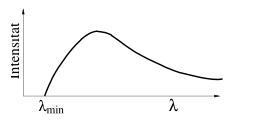
\includegraphics{images/kontinuirlich.png}
  \caption{Beispiel für ein kontinuirliches Bremsspektrum.\cite{sample}}
  \label{fig:kontinuirlich}
\end{figure}
Die minimale Wellenlänge ${\lambda}_\text{min}$, und damit die maximal mögliche Energie der Röntgenstrahlung wird durch die Energieerhaltung zu folgendem Ausdruck bestimmt:
\begin{equation}
  {\lambda}_\text{min} = \frac{h \cdot c}{e_0 U} .
  \label{eqn:lambdamin}
\end{equation}
Dabei ist $h$ das Plancksche Wirkungsquantum, $c$ die Lichtgeschwindigkeit, $e_0$ die Elementarladung und $U$ die angelegte Spannung.
Zusätzlich zum Bremsspektrum wird aber auch ein materialspezifisches charakteristisches Spektrum des Anodenmaterials beobachtet. Dies entsteht durch das herauslösen eines
Elektrons aus einer inneren Atomschale durch das beschleunigte Elektron. Da das Atom den energetisch niedrigsten Zustand annehmen will, besetzt ein Elektron aus einer höheren
Schale den frei gewordenen Platz. Da dieses Elektron dabei von einem Zustand höherer Energie in einen Zustand niedriger Energie wechselt, wird wieder Energie in Form von
Strahlung frei. Da die Energieniveaus der einzelnenen Atomschalen, und somit auch die Energiedifferenzen dieser feste Energiewerte besitzen, entsteht ein Linienspektrum. Die
Linien werden nach der Schale auf welchem das Elektron herausgelöst wurde und einem grieschichen Buchstaben, welcher die Herkunft des auffüllenden Elektrons beschreibt, bennant.
Ein Beispiel wäre $K_{\alpha}$. Gerade in größeren Atomen muss jedoch bei der Energie der Schalen die Abschirmung durch die inneren Elektronenhüllen berücksichtigt werden, indem
eine effektive Kernladung $z_\text{eff}= z - \sigma$, mit der Abschirmkonstante $\sigma$ eingeführt wird. Die Bindungsenergie eines Elektrons kann dann mit
\begin{equation}
  E_n = - R_{\infty} {z_\text{eff}}^2 \cdot \frac{1}{n^2}
  \label{eqn:En}
\end{equation}
berechnet werden. $R_{\infty} = \SI{13.6}{\electronvolt}$ ist hierbei die Rydbergenergie. Aus den Differenzen der jeweiligen Energieniveaus der beteiligten Schalen kann dann die
Energie der Röntgenstrahlung berechnet werden.
Für die Abschirmkonstante ergibt sich durch Umstellen folgender Ausdruck:
\begin{equation}
  \sigma = Z-\sqrt{\frac{E_n}{R_{\infty}}}\cdot n .
  \label{eqn:sigma}
\end{equation} \\\\
Bei der Absorption von Röntgenstrahlung unter $\SI{1}{\mega\electronvolt}$ treten hauptsächlich der Photo- und Comptoneffekt auf. Bei steigender Energie nimmt der Absorptionskoeffizient
ab, zeigt jedoch einen Sprunghaften Anstieg bei bestimmten Energien. Dies ist in Abbildung \ref{fig:absorption} zu sehen.
\begin{figure}
  \centering
  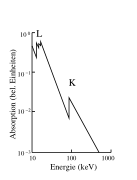
\includegraphics{images/absorption.png}
  \caption{Beispiel für ein Absorptionsspektrum.\cite{sample}}
  \label{fig:absorption}
\end{figure}
Diese Anstiege entstehen durch das herauslösen eines Elektrons aus der nächsten höheren Schale.
Somit ist die Lage dieser sogennanten Absorptionskanten nahe der Bindungsenergie der Elektronen. Die Kanten werden ähnlich wie die Emissionslinien nach der jeweiligen Schale
benannt und bei weiterer Aufteilung durch die Feinstruktur einfach druchnummeriert. SO gibt es zum Beispiel die $L_I$, $L_{II}$ und $L_{III}$ Kante. Quantitativ wird
die Absorptionskante durch
\begin{equation}
  h \cdot {\nu}_\text{Abs} = E_n - E_{\infty}
  \label{eqn:kante}
\end{equation}
und die Bindungsenergie der Elektronen durch
\begin{equation}
  E_\text{n,j} = - R_{\infty} \Biggl({z_\text{eff,1}}^2 \cdot \frac{1}{n^2} + {\alpha}^2 {z_\text{eff,2}}^4 \cdot \frac{1}{n^3} \Biggl(\frac{1}{j+\sfrac{1}{2}} - \frac{3}{4n} \Biggr) \Biggr)
  \label{eqn:feinstruktur}
\end{equation}
mit der Sommerfeldschen Feinstrukturkonstante $\alpha$ und dem Gesamtdrehimpuls des Elektrons $j$.
Zur Berechnung der Abschirmkonstanten aus der L-Kante kann durch das fehlende Auflösungsvermögen der Messapparatur mithilfe der Energiedifferenz $\Delta E_L = E_{L_{II}}- E_{L_{III}}$ folgender
Ausruck hergeleitet werden:
\begin{equation}
{\sigma}_L = Z - \Biggl(\frac{4}{\alpha} \sqrt{\frac{\Delta E_L}{R_{\infty}}} - \frac{5 \Delta E_L}{R_{\infty}} \Biggr)^{1/2} \Biggl(1+ \frac{19}{32} {\alpha}^2 \frac{\Delta E_L}{R_{\infty}} \Biggr)^{1/2} .
\label{eqn:sigmaL}
\end{equation}
Zur experimentellen Untersuchung der Röntgenstrahlung wird die Braggsche Reflexion ausgenutzt. Dabei wird das Röntgenlicht an einem dreidimensionalen Gitter, zum Beispiel einem Kristall, gebeugt.
Dies ist in Abbildung \ref{fig:braggreflexion} zu sehen.
\begin{figure}
  \centering
  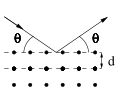
\includegraphics{images/bragg.png}
  \caption{Schematische Darstellung der Bragg-Reflexion.\cite{sample}}
  \label{fig:braggreflexion}
\end{figure}
Beim Glanzwinkel $\theta$ wird eine konstruktive Interferenz und somit ein Maximum der Intensität beobachtet. So lässt sich aus dem Beugungswinkel $\theta$ und der Gitterkonstanten $d$ mit
\begin{equation}
  2 \, d \, \sin{\theta} = n \, \lambda
  \label{eqn:bragg}
\end{equation}
die gebeugte Wellenlänge $\lambda$ und somit auch die Energie der Strahlung bestimmen.
Wird dies nun für $n = 1$ in die Gleichung \eqref{eqn:lambdamin} eingesetzt und nach der Energie umgestellt, ergibt sich folgender Ausdruck:

\begin{equation}
  E = \frac{h c}{2 d \sin{\theta}}
  \label{eqn:Energie}
\end{equation}
